% Source for docs/static/img/mapl-iterative.svg. Rebuild from the repository root:
%   pdflatex -output-directory=/tmp docs/scripts/mapl-iterative.tex
%   pdf2svg /tmp/mapl-iterative.pdf docs/static/img/mapl-iterative.svg
%   python3 docs/scripts/prepare_rollout_svgs.py
% Keep the stage boundaries in prepare_rollout_svgs.py in sync with the row positions.
% Shared preamble for the CoMLRL training-flow diagrams. Paste it verbatim at the
% top of every diagram so each .tex stays standalone.
\documentclass[tikz,border=3pt]{standalone}
\usepackage{amsmath,amssymb,bm}
\usetikzlibrary{arrows.meta,positioning,calc,fit}

% Only these paints have dark-theme mappings (assets/_diagram-theme.scss).
\colorlet{agentA}{red!80!black}     % agent 1: policy, prompts, responses, loss
\colorlet{agentB}{blue!80!black}    % agent 2
\colorlet{learned}{orange!80!black} % learned evaluators: critic, reward model
\colorlet{update}{green!50!black}   % gradients and parameter updates
% Joint or shared quantities are black. Gray = black with fill opacity.

\tikzset{
  >={Stealth[length=3.2pt,width=3pt]},
  box/.style={draw, line width=1pt, inner sep=2.5pt, minimum height=13pt},
  policy/.style={box, rounded corners=3pt, minimum width=30pt},
  flow/.style={->, line width=.8pt},
  note/.style={font=\scriptsize, align=left},
  label/.style={anchor=west, font=\footnotesize},
}


% One iteration nu of the iterative preference trainers, unrolled top to bottom.
% Rows are animation stages; avoid \frac and \_ (their rules animate as edges).
\begin{document}
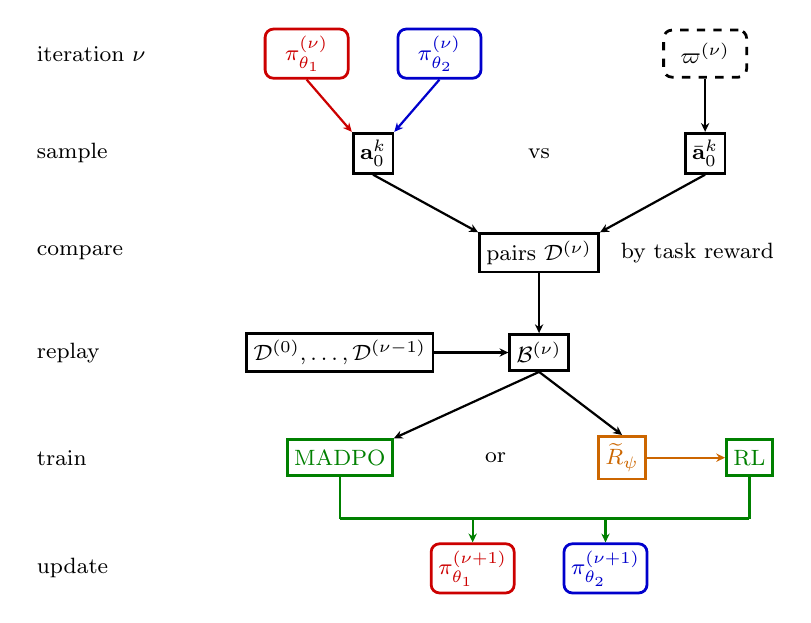
\begin{tikzpicture}[x=1pt, y=1pt, font=\footnotesize,
    top/.style={minimum height=17pt}]
  \def\xa{125}  % current policies (center of the pair)
  \def\xc{185}  % shared column
  \def\xq{245}  % comparator

  % Stage 0: current policies and the comparator.
  \node[label] at (0,0) {iteration $\nu$};
  \node[policy, top, agentA] (p1) at (\xa-24,0) {$\pi^{(\nu)}_{\theta_1}$};
  \node[policy, top, agentB] (p2) at (\xa+24,0) {$\pi^{(\nu)}_{\theta_2}$};
  \node[policy, top, dashed] (q) at (\xq,0) {$\varpi^{(\nu)}$};

  % Stage 1: both sides sample candidate k.
  \node[label] at (0,-36) {sample};
  \node[box] (a) at (\xa,-36) {$\mathbf{a}^k_0$};
  \node[box] (b) at (\xq,-36) {$\bar{\mathbf{a}}^k_0$};
  \draw[flow, agentA] (p1.south) -- (a.north west);
  \draw[flow, agentB] (p2.south) -- (a.north east);
  \draw[flow] (q) -- (b);
  \node at (\xc,-36) {vs};

  % Stage 2: the task reward orders each pair; pairs form this round's dataset.
  \node[label] at (0,-72) {compare};
  \node[box] (D) at (\xc,-72) {pairs $\mathcal{D}^{(\nu)}$};
  \draw[flow] (a.south) -- (D.north west);
  \draw[flow] (b.south) -- (D.north east);
  \node[anchor=west] at ([xshift=4pt]D.east) {by task reward};

  % Stage 3: replay selects the training pairs from this and earlier rounds.
  \node[label] at (0,-108) {replay};
  \node[box] (B) at (\xc,-108) {$\mathcal{B}^{(\nu)}$};
  \node[box] (H) at (\xa-12,-108) {$\mathcal{D}^{(0)},\ldots,\mathcal{D}^{(\nu-1)}$};
  \draw[flow] (D) -- (B);
  \draw[flow] (H) -- (B);

  % Stage 4: MADPO, or a reward model followed by RL.
  \node[label] at (0,-146) {train};
  \node[box, update] (m) at (\xa-12,-146) {MADPO};
  \node[box, learned] (r) at (\xc+30,-146) {$\widetilde{R}_{\psi}$};
  \node[box, update] (o) at (\xc+76,-146) {RL};
  \draw[flow, learned] (r) -- (o);
  \draw[flow] (B.south) -- (m.north east);
  \draw[flow] (B.south) -- (r.north);
  \node at ($(m.east)!.5!(r.west)$) {or};

  % Stage 5: the updated policies start iteration nu+1.
  \def\yb{-168}
  \node[label] at (0,-186) {update};
  \node[policy, top, agentA] (n1) at (\xc-24,-186) {$\pi^{(\nu+1)}_{\theta_1}$};
  \node[policy, top, agentB] (n2) at (\xc+24,-186) {$\pi^{(\nu+1)}_{\theta_2}$};
  \draw[update, line width=.8pt] (m.south) -- (m.south |- 0,\yb);
  \draw[update, line width=.8pt] (o.south) -- (o.south |- 0,\yb);
  \draw[update, line width=.8pt] (m.south |- 0,\yb) -- (o.south |- 0,\yb);
  \foreach \n in {n1,n2} \draw[flow, update] (\n.north |- 0,\yb) -- (\n.north);
\end{tikzpicture}
\end{document}
